% sample main.tex created 2015-03-26 by bob jantzen
\documentclass{ws-procs975x65}
% optional packages

\usepackage[T1]{fontenc}
\usepackage[utf8]{inputenc}
\usepackage{graphicx}
\usepackage{xspace}


%%%%%%%%%%%%%%%%%%%%%%%%%%%%%%%%%%%%%%%%%%%%%%%%%%%%%%%%%%%%%%%%%%%%%%%%%%%%%%%%%
% a few author defined macros like:
%\def\beq{\begin{equation}}
%\def\eeq{\end{equation}}

%%%%%%%%%%%%%%%%%%%%%%%%%%%%%%%%%%%%%%%%%%%%%%%%%%%%%%%%%%%%%%%%%%%%%%%%%%%%%%%%%

% shortcuts for pubs
\newcommand{\apj}{ApJ}
\newcommand{\apjs}{ApJS}
\newcommand{\apjl}{ApJL}
\newcommand{\aap}{A{\&}A}
\newcommand{\aaps}{A{\&}AS}
\newcommand{\mnras}{MNRAS}
\newcommand{\aj}{AJ}
\newcommand{\araa}{ARAA}
\newcommand{\pasp}{PASP}
\newcommand{\pasj}{PASJ}
\newcommand{\nat}{Nature}
\newcommand{\nar}{New Astr Rev}


% makes it easier to have consistent writing, and easy change if needed
\newcommand{\spl}{SpaghettiLens\xspace}
\newcommand{\sw}{Space Warps\xspace}

\newcommand{\Msun}{\ensuremath{\text{M}_\odot}\xspace}

\newcommand{\Mlens}{\ensuremath{\text{M}_\text{lens}}\xspace}
\newcommand{\Mstel}{\ensuremath{\text{M}_\odot}\xspace}

% shortcut for einstein radius (Text Greek Full Math)
\newcommand{\ERf}[1][]{$\Theta_\text{E#1}$\xspace} % full output
%\newcommand{\ER}{Einstein radius\xspace} % text
%\newcommand{\ERg}[1][]{$\Theta_{\text{E#1}}$\xspace} % er in textmode with greek
%\newcommand{\ERm}[1][]{\Theta_\text{E#1}} % mathmode with greek symbol
%\newcommand{\kenc}[1][r]{$\kappa_\text{encl}(#1)$\xspace}
%\newcommand{\kap}[1][r]{$\kappa(#1)$\xspace}

% shorcuts for refs and citations
\newcommand{\icite}[1]{Ref.~\refcite{#1}} % *I*nline citation
\newcommand{\scite}[1]{\cite{#1}} % end of *S*entence citation

\newcommand{\figref}[1]{Figure~\ref{fig:#1}}

%\newcommand{\fref}[1]{\ref{fig:#1}}
%\newcommand{\sref}[1]{\ref{sec:#1}}
%\newcommand{\tref}[1]{\ref{tab:#1}}
%\newcommand{\secref}[1]{Section~\ref{sec:#1}}
%\newcommand{\tabref}[1]{Table~\ref{tab:#1}}
%\newcommand{\Figref}[1]{Figure~\ref{fig:#1}}
%\newcommand{\Secref}[1]{Section~\ref{sec:#1}}
%\newcommand{\Tabref}[1]{Table~\ref{tab:#1}}


% shortcut for ASW000xxxx
\newcommand{\asw}[1]{ASW000#1\xspace}
\newcommand{\model}[2][Model~]{#1#2\xspace}


\newcommand{\dgr}{^{\circ}}
\newcommand{\tgeom}{t_{\rm geom}}
\newcommand{\tgrav}{t_{\rm grav}}
\newcommand{\subcirc}{{\lower.33ex\hbox{$\circ$}}}
\newcommand{\subbullet}{{\lower.33ex\hbox{$\bullet$}}}




\begin{document}



\title{Lensing Galaxies in the CFHT Legacy Survey}

\author{
  Rafael Küng$^*$, Prasenjit Saha
}
\address{
Physik-Institut, University of Zürich,\\
Winterthurerstrasse 190, 8057 Zürich, Switzerland\\
$^*$E-mail: rafael\_kueng@uzh.ch
}
\author{
  Anupreeta More, Surhud More
}
\address{
  Kavli Institute for the Physics and Mathematics of the Universe, University of Tokyo\\ 5-1-5 Kashiwanoha, Kashiwa-shi 277-8583, Japan
}

\author{
  Elisabeth Baeten, Claude Cornen, Christine Macmillan, Julianne K. Wilcox
}
\address{
  Zooniverse, c/o Astrophysics Department, University of Oxford\\
  Oxford OX1 3RH, UK
}

\author{
  Jonathan Coles
}
\address{
  Exascale Research Computing Lab, Campus Teratec,\\
  2 Rue de la Piquetterie, 91680 Bruyeres-le-Chatel, France
}

\author{Ignacio Ferreras}
\address{Mullard Space Science Laboratory, University College London, Holmbury St Mary, Dorking, Surrey RH5 6NT, UK}

\author{
  Phil Marshall
}
\address{
  Kavli Institute for Particle Astrophysics and Cosmology, Stanford University\\
  452 Lomita Mall, Stanford, CA 94035, USA
}

\author{
  Aprajita Verma
}
\address{
  Sub-department of Astrophysics, University of Oxford, Denys Wilkinson Building\\
  Keble Road, Oxford, OX1 3RH, UK
}





% \title{Short Sample Template File for MG14: \\ Include Full First Names}
% \author{Andrew B. Author$^*$ and Charles D. Author}
% 
% \address{University Department, University Name,\\
% City, State ZIP/Zone, Country\\
% $^*$E-mail: ab\_author@university.com\\
% www.university\_name.edu}
% 
% \author{Anthony N. Author} 
% 
% \address{Group, Laboratory, Street,\\
% City, State ZIP/Zone, Country\\
% E-mail: an\_author@laboratory.com}





\begin{abstract}
In SpaceWarps, a community of over 30'000 volunteers searched for lensed candidates
in the CFHT Legacy Survey. About 60 new lens candidates have been identified, along
with rediscovery of 60\% of the previously-known candidates.

Models of most of these lens candidates were produced collaboratively by a small
community of lens enthusiasts from the volunteer community. Tests with simulated
lenses show that models by experienced volunteers are comparable to those by
experts.

We will present lens models of some these newly discovered lens candidates, along
with a modelling method developed to be usable in a citizen-science environment.
Preliminary results comparing stellar and lensing masses will also be
presented.
\end{abstract}


\keywords{Gravitational Lensing: strong; methods: numerical; MG14 Proceedings}


\bodymatter

%%%%%%%%%%%%%%%%% now a standard article style for the most part


\section{Introduction}

Gravitational lenses (GL), prediced by A. Einstein's General Relativity in 1915 have become an important tool in cosmology.
Strong lensing can be used to infer the distribution of dark matter around galaxies (e.g. \icite{Koopans2009}), to find the relation between stars and dark matter (\icite{Leier2011}) or to infer cosmological parameters (\icite{Sereno2014}).

Current surveys resulted in a few hundred of known lenses.
For example in the Space Warps project (\icite{sw1,sw2}), carried out on the 170 square degree Canada--France--Hawaii Telescope Legacy Survey (CFHTLS), over 30'000 volunteers found 59 candidate lenses.
As a rough estimate, this is one lens every few square degree.

Imaging surveys under way will increase the observation area by a factor of ten and next gen surveys starting in the twenty-twenties will increase the resolution by another factor of ten.\scite{Marshall2005,OguriMarshall2010}
This raises expectations that the number of lenses will increase a hundred fold, leading to an order of 10'000 lenses over the next 10 years.
Thats of order one possible lens detection per hour.







\begin{itemize}
  \item NOW:
  \item CHFT LS: 150 deg$^2$
  \item 50000 volunteers, 11mio classifications
  \item 59 candidates found
  \item 1 lens every few deg$^2 $
  \item FUTURE:
  \item DES Pan-STARRS (x10); LSST, Euclid (2020+, again x10)
  \item leads to 10'000 lenses over next 10 years
  \item order of one per hour
\end{itemize}

Detecting lenses: robots + \sw

post processing (modelling): robots? no; citicen science!

Theory (short summary from \icite{Kueng2015})

Arrival time / Time delay.
\begin{equation}  \label{eq:tarriv}
t(x,y) = t_{\rm geom} + t_{\rm grav}
\end{equation}

With the geometrical time delay / change of flight path
\begin{equation} \label{eq:tgeom}
\tgeom(x,y) \propto (x-x_s)^2 + (y-y_s)^2 ,
\end{equation}

And the delay due to general relativity
\begin{equation} \label{eq:tgrav}
\tgrav(x,y) = \left\langle \tgrav(x_\subcirc,y_\subcirc) \right\rangle
              + (1+z_L) \frac{2G}{c^3} M(x_\subbullet,y_\subbullet) \,.
\end{equation}

t(x,y) is an arrival time countour
can be modelled by skeching self intersecting contour lines.
Sampling techique described in detail in \icite{Lubini2012}.
A spaghetti lens model is en ensemble of 200 models, uncertainty is the range covered by the ensemble.




\section{Creating and Selecting Modells}

describe modelling tree

\begin{figure}
  \centering
  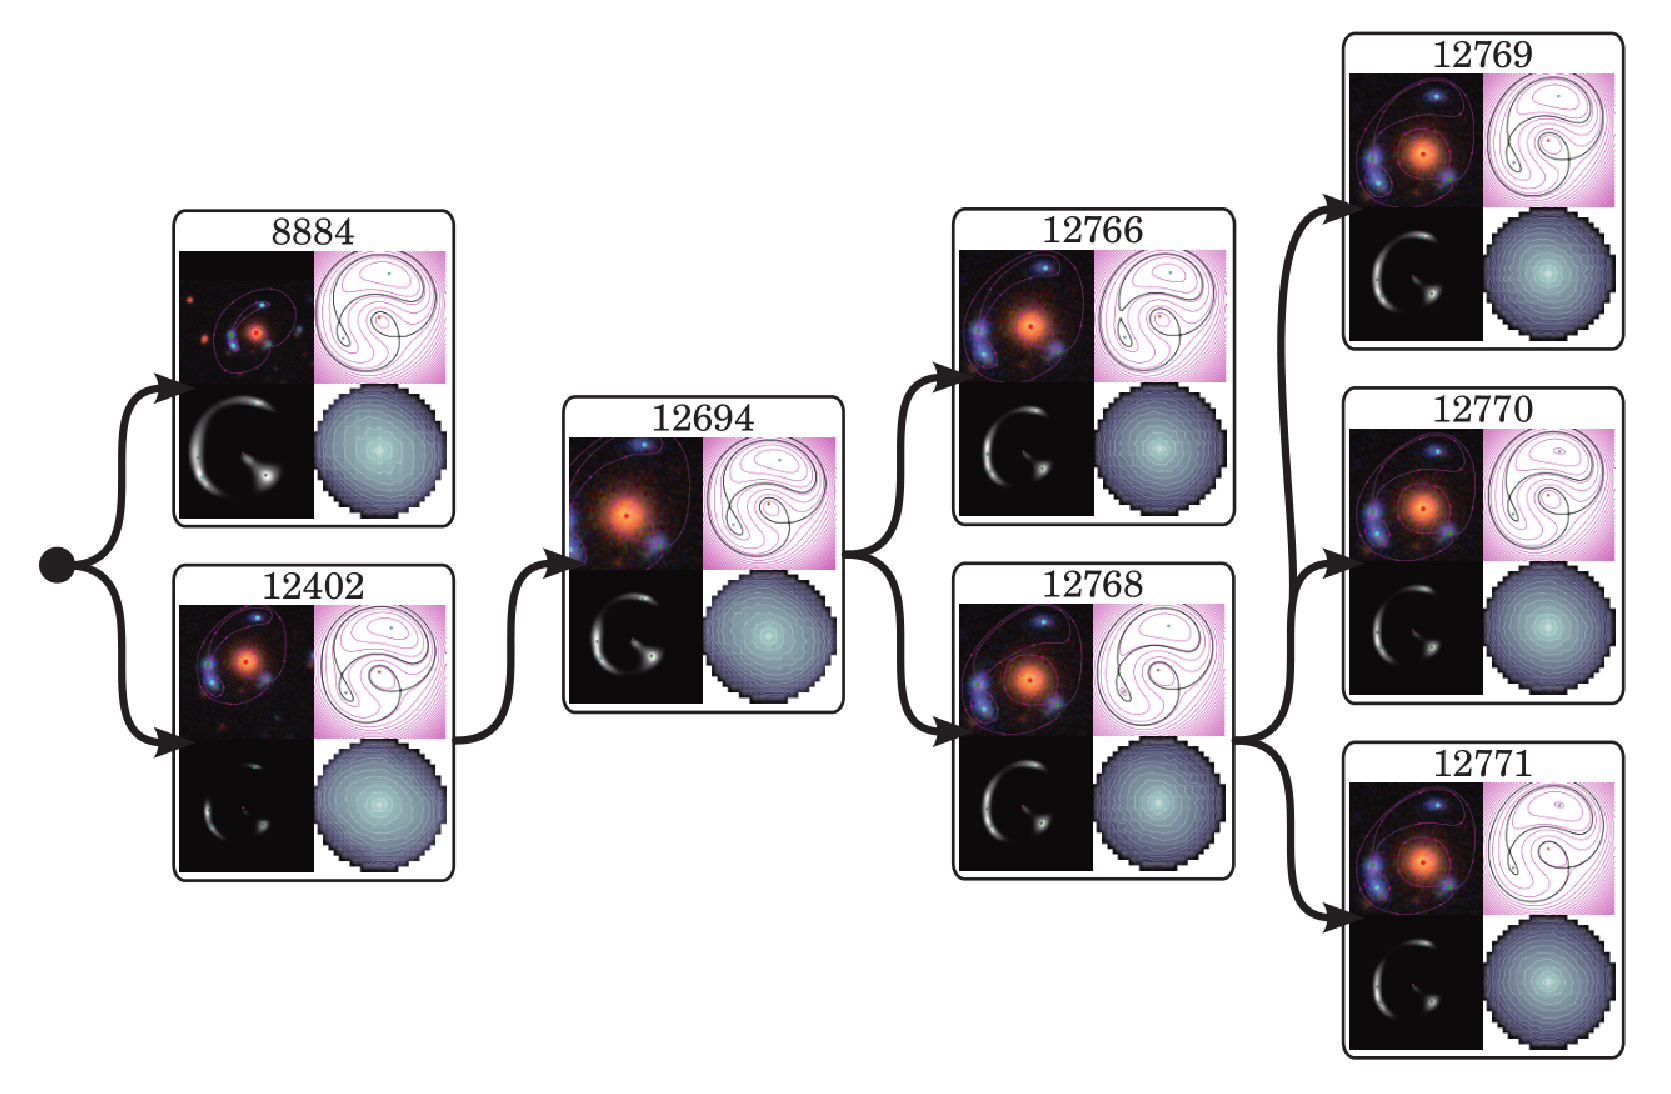
\includegraphics[width=0.8\columnwidth]{img/modeltree}
  \caption{
    modelltree
  }
  \label{fig:tree}
\end{figure}

for this analysis, models from the tree were selected manually by inspection by PS, RK and the community.


\section{Determing Lensing and Stellar Mass}

The lensing mass can directly be extracted from the generated models, as the mass distribution is the key feature that is being modelled (\icite{Kueng2015}).
Since a single model actually consists of an ensemble of a number of models, where each one is a possible configuration, we get an approximation of the error by selecting the models with minimal/ maximal total mass as lower / upper bounds for the errors.

We estimated the stellar mass with:
\[
  \Mstel = 10^{0.4 [\operatorname{mag}(z_\text{ph}) - m_\text{i}]}
\]
where
$z_\text{ph}$ and $m_\text{i}$ are the photometric redshift and luminosity given in \icite{sw2} and 
$\operatorname{mag}()$ is a function obtained by interpolating data of SDSS-i magnitude (AB) of 1\Msun and actual mass vs redshift BC03 models (\icite{Bruzual2003}), Salpeter Initial Mass Function and assumes ``vanilla cosmology'' ($\Omega_\text{M}=0.3$, $\Omega_\Lambda=0.7$).\scite{Ferreras2010}
For the lower bound of the error we assumed a young population (0.5 Gyr), whereas for the upper one of 2 Gyr.


\section{Conclusions}

In this work we use the method presented and tested in \icite{Kueng2015} to create models of all lens candidates discovered by \icite{sw2}.
We determine the total (lensing) mass \Mlens of the candidates using the generated models and the stellar mass \Mstel using an interpolation of a Salpeter Initial Mass Function (\icite{Salpeter1955}) with redshifts and luminosity magnitudes given in \icite{sw2}.
We then plot the masses of the candidates and observe in \figref{frac} that the stellar mass fraction is of the order of 20\%, with decreasing trend for the most massive galaxies, as expected for early type galaxies.
We identify outliers with very low stellar masses that need further inspection.

\begin{figure}
  \centering
  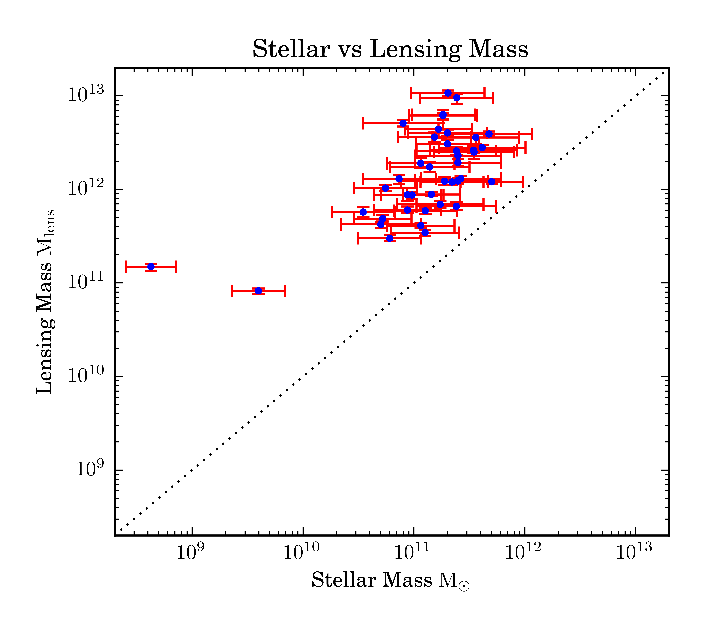
\includegraphics[width=0.8\columnwidth]{img/plot}
  \caption{Stellar Mass \Mstel vs. Lensing Mass \Mlens. Stellar Mass errors are the difference between junior (0.5 Gyr) and senior (2 Gyr) population; Lensing Mass errors represent the minimum and maximum values of an ensemble (``a model'').}
  \label{fig:frac}
\end{figure}


\section*{Acknowledgments}
RK thanks the Candoc Grant (UZH Forschungskredit) for their support of this work.

\bibliographystyle{ws-procs975x65}
\bibliography{ms}



% \section{The First Section: Titles are Capitalized with the Usual First Letter Rules}
% \subsection{Subsections only have the first letter of the entire title capitalized}
% 
% Subsections only have the first letter of the first word capitalized (except for words that are naturally capitalized). For a very short contribution it is not necessary to use the sectioning commands.
% 
% You may also use the ``graphicx" package and use its related commands if you are already familiar with that figure insertion method. Word template files are discouraged, allowed as a last resort for those people who have some difficulties with \LaTeX.
% 
% Since the World Scientific proceedings style \cite{ws} uses numbered superscript citations of the bibliography items, one has to be careful to use 
% \verb|\refcite| to get a baseline normal size number to include in an in-line direct reference, best formatted in the style: 
%  ``see Ref.$\sim$\verb|\refcite|\{\ldots\}" while normal superscript citations follow punctuation  as in ``.\verb|\cite|\{\ldots\}"  For example, here is an in line citation to Ref.~\refcite{arxiv}. On the other hand citations at the end of a sentence are done line this.\cite{lamp94}
% 
% \subsection{You can safely ignore this}
% 
% The white space above the title in the ws-procs975x65.cls document style is eliminated by commenting out two lines in the definition of the macro \verb|\title|, namely:\\  
%  \verb|\vspace|*\{-14pt\} \\ \verb|\vskip| 59pt\\
% but you do not need to know this if you use the proceedings style files downloaded from the MG14 website. This gives a bit more space for text content in short articles.
% 
% For MG14 \cite{mg14} only a preview PDF document will be collected (exported from your \LaTeX\ document) before the meeting takes place.
% 
% \section*{Acknowledgments}
% 
% What a debt we all owe to Donald Knuth for his gift of \TeX\ to us and to Leslie Lamport as well for its \LaTeX\ child.



\end{document}

